% Preamble
\documentclass[11pt, aspectratio=169]{beamer}
	% Packages
	\usepackage[english]{babel}
	\usepackage{lipsum}
	\usepackage{mathptmx}
	\usepackage{xcolor}
	\usepackage{amsmath, amssymb, amsthm}
	\usepackage{graphics}
	\usepackage{float}
	\usepackage{hyperref}
	% Themes
	\usefonttheme[onlymath]{serif}
	\usetheme[nofirafonts]{focus}
	\renewcommand{\thempfootnote}{\arabic{mpfootnote}}
	% Cover
	\title{Microeconometrics Using Stata}
	\subtitle{Simulation}
	\author{
		Jhon R. Ordoñez
		\footnote{\label{1} National University of San Cristóbal de Huamanga}
		\footnote{\label{2} Faculty of Economic, Administrative and Accounting Sciences}
		\footnote{\label{3} Professional School of Economics}
	}
	\date{\today}
% Body
\begin{document}
	% Cover
	\begin{frame}
		\maketitle
	\end{frame}
	% Outline
	\begin{frame}[t]
		\frametitle{Outline}
		\tableofcontents
	\end{frame}
	% Section 1
	\section{Exercise 1}
		% Slide 1
		\begin{frame}
			\frametitle{Exercise 1}
				\begin{block}{Exercise 1}
					Give the commands \textcolor{blue}{\textbf{set obs 100}} and \textcolor{blue}{\textbf{generate u = runiform()}} and
					\textcolor{blue}{\textbf{summarize}}. Then, give command \textcolor{blue}{\textbf{clear}} and repeat the initial
					commands. Did you get the same result? If not, explain why, and adapt
					your code to get the same results.
				\end{block}
		\end{frame}
	% Section 2
	\section{Exercise 2}
		% Slide 1
		\begin{frame}
			\frametitle{Exercise 2}
			\begin{block}{Exercise 2}
				Using the normal generator, generate a random draw from a $50-50$
				scale mixture of $N(1,1)$ and $N(1,3^{2})$ distributions. Repeat the
				exercise with the $N(1,3^{2})$ component replaced by $N(3,1)$. For both
				cases, display the features of the generated data by using a kernel
				density plot.
			\end{block}
		\end{frame}
	% Section 3
	\section{Exercise 3}
		% Slide 1
		\begin{frame}
			\frametitle{Exercise 3}
			\begin{block}{Exercise 3}
				Generate $1,000$ observations from the $F(5,10)$ distribution. Use
				\textcolor{blue}{\textbf{rchi2()}} to obtain draws from the $\chi^{2}(5)$ and the $\chi^{2}(10)$ distributions.
				Compare the sample moments with their theoretical counterparts.
			\end{block}
		\end{frame}
	% Section 4
	\section{Exercise 4}
		% Slide 1
		\begin{frame}
			\frametitle{Exercise 4}
			\begin{block}{Exercise 4}
				Make $1,000$ draws from the $N(6,2^{2})$ distribution by making a
				transformation of draws from $N(0,1)$ and then making the
				transformation $Y = \mu + \sigma Z$.
			\end{block}
		\end{frame}
	% Section 5
	\section{Exercise 5}
		% Slide 1
		\begin{frame}
			\frametitle{Exercise 5}
			\begin{block}{Exercise 5}
				Generate $1,000$ draws from the $t(6)$ distribution, which has a mean of
				$0$ and a variance of $4$. Compare your results with those from
				\textbf{exercise 4}.
			\end{block}
		\end{frame}
	% Section 6
	\section{Exercise 6}
		% Slide 1
		\begin{frame}
			\frametitle{Exercise 6}
			\begin{block}{Exercise 6}
				Generate a large sample from the $N(\mu = 1, \sigma^{2} = 1)$ distribution and
				estimate $\sigma/\mu$ , the coefficient of variation (\textbf{CV}). Verify that the sample
				estimate is a consistent estimate.
			\end{block}
		\end{frame}
	% Section 7
	\section{Exercise 7}
		% Slide 1
		\begin{frame}
			\frametitle{Exercise 7}
			\begin{block}{Exercise 7}
				Generate a draw from a multivariate normal distribution,
				$N(\mathbf{\mu}, \Sigma = \mathbf{LL'})$, with $\mathbf{\mu'} = [0x0x0]$ and 
					\begin{equation}
						\mathbf{L} = \left[
							\begin{matrix}
								1 & 0 & 0 \\
								1 & \sqrt{3} & 0\\
								0 & \sqrt{3} & \sqrt{6}
							\end{matrix}
						\right], \text{or}\quad \Sigma = \left[
							\begin{matrix}
								1 & 1 & 0 \\
								1 & 4 & 3 \\
								0 & 3 & 9
							\end{matrix}
						\right]
					\end{equation}
				using transformations based on this Cholesky decomposition. Compare
				your results with those based on using the \textcolor{blue}{\textbf{drawnorm}} command.
			\end{block}
		\end{frame}
	% Section 8
	\section{Exercise 8}
		% Slide 1
		\begin{frame}[t]
			\frametitle{Exercise 8}
			\begin{block}{Exercise 8}
				Let $s$ denote the sample estimate of $\sigma$ and $\bar{x}$ denote the sample
				estimate of $\mu$. The \textbf{CV} $\sigma/\mu$ , which is the ratio of the standard deviation
				to the mean, is a dimensionless measure of dispersion. The asymptotic
				distribution of the sample \textbf{CV} $s/\bar{x}$ is 
					\begin{equation}
						N\left\{\dfrac{\sigma}{\mu} , \left(N-2\right)^{-\dfrac{1}{2}}\left(\dfrac{\sigma}{\mu}\right)^{2}\left[ 0.5 + \left(\dfrac{\sigma}{\mu}\right)^{2}  \right] \right\}       
					\end{equation}
				see \textcolor{red}{\textbf{Miller (1991)}}. For $N = 25$, using either \textcolor{blue}{\textbf{simulate}} or \textcolor{blue}{\textbf{postfile}}, compare the Monte Carlo
				and asymptotic variance of the sample \textbf{CV} with the following
				specification of the \textbf{DGP}: $x \sim N(\mu, \sigma^{2})$ with three different values of
				\textbf{CV} $= 0.1 , 0.33,$ and $0.67$.
			\end{block}
		\end{frame}
	% Section 9
	\section{Exercise 9}
		% Slide 1
		\begin{frame}
			\frametitle{Exercise 9}
			\begin{block}{Exercise 9}
				It is suspected that making draws from the truncated normal using the
				method given in \textcolor{red}{\textbf{section 5.4.4}} may not work well when sampling from
				the extreme tails of the normal. Using different truncation points,
				check this suggestion.
			\end{block}
		\end{frame}
	% Section 10
	\section{Exercise 10}
		% Slide 1
		\begin{frame}[t, label = Slide 1]
			\frametitle{Exercise 10}
			\begin{block}{Exercise 10}
				Repeat the example of \textcolor{red}{\textbf{section 5.6.1}} (OLS with $\chi^{2}$ errors), now using
				the \textcolor{blue}{\textbf{postfile}} command. Use \textcolor{blue}{\textbf{postfile}} to save the estimated slope
				coefficient, standard error, the $t$ statistic for $H_{0}: \beta = 2$, and an
				indicator for whether $H_{0}$ is rejected at the $0.05$ level in a Stata file
				named \textcolor{blue}{\textbf{simresults}}. The template program is as follows
				(\hyperlink{Slide 1 see template}{\beamergotobutton{see template}}):
			\end{block}
		\end{frame}
	% References
	\begin{frame}[t,allowframebreaks]
		\frametitle{References}
		\bibliography{biblio.bib}
		% Style
		\bibliographystyle{apalike}
		% Authors
		\nocite{cameron2022-I}
		\nocite{cameron2022-II}
	\end{frame}
	% Cover
	\begin{frame}
		\maketitle
	\end{frame}
	% Appendix
	\begin{frame}[t, label = Slide 1 see template]
		\begin{block}{\hyperlink{Slide 1}{\beamergotobutton{back}}}
			\begin{figure}[H]
				\centering
				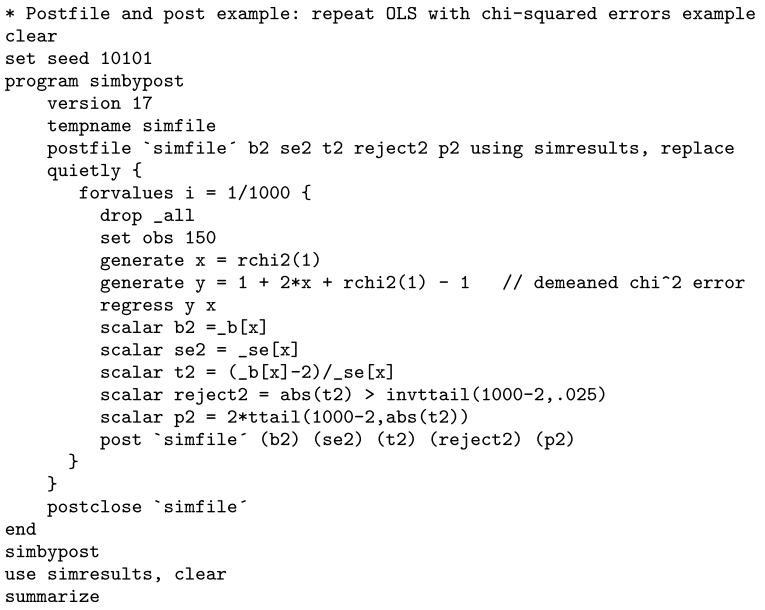
\includegraphics[scale=0.42]{figures/fig1.PNG}
			\end{figure}
		\end{block}
	\end{frame}
\end{document}